\begin{figure}[!htbp]\centering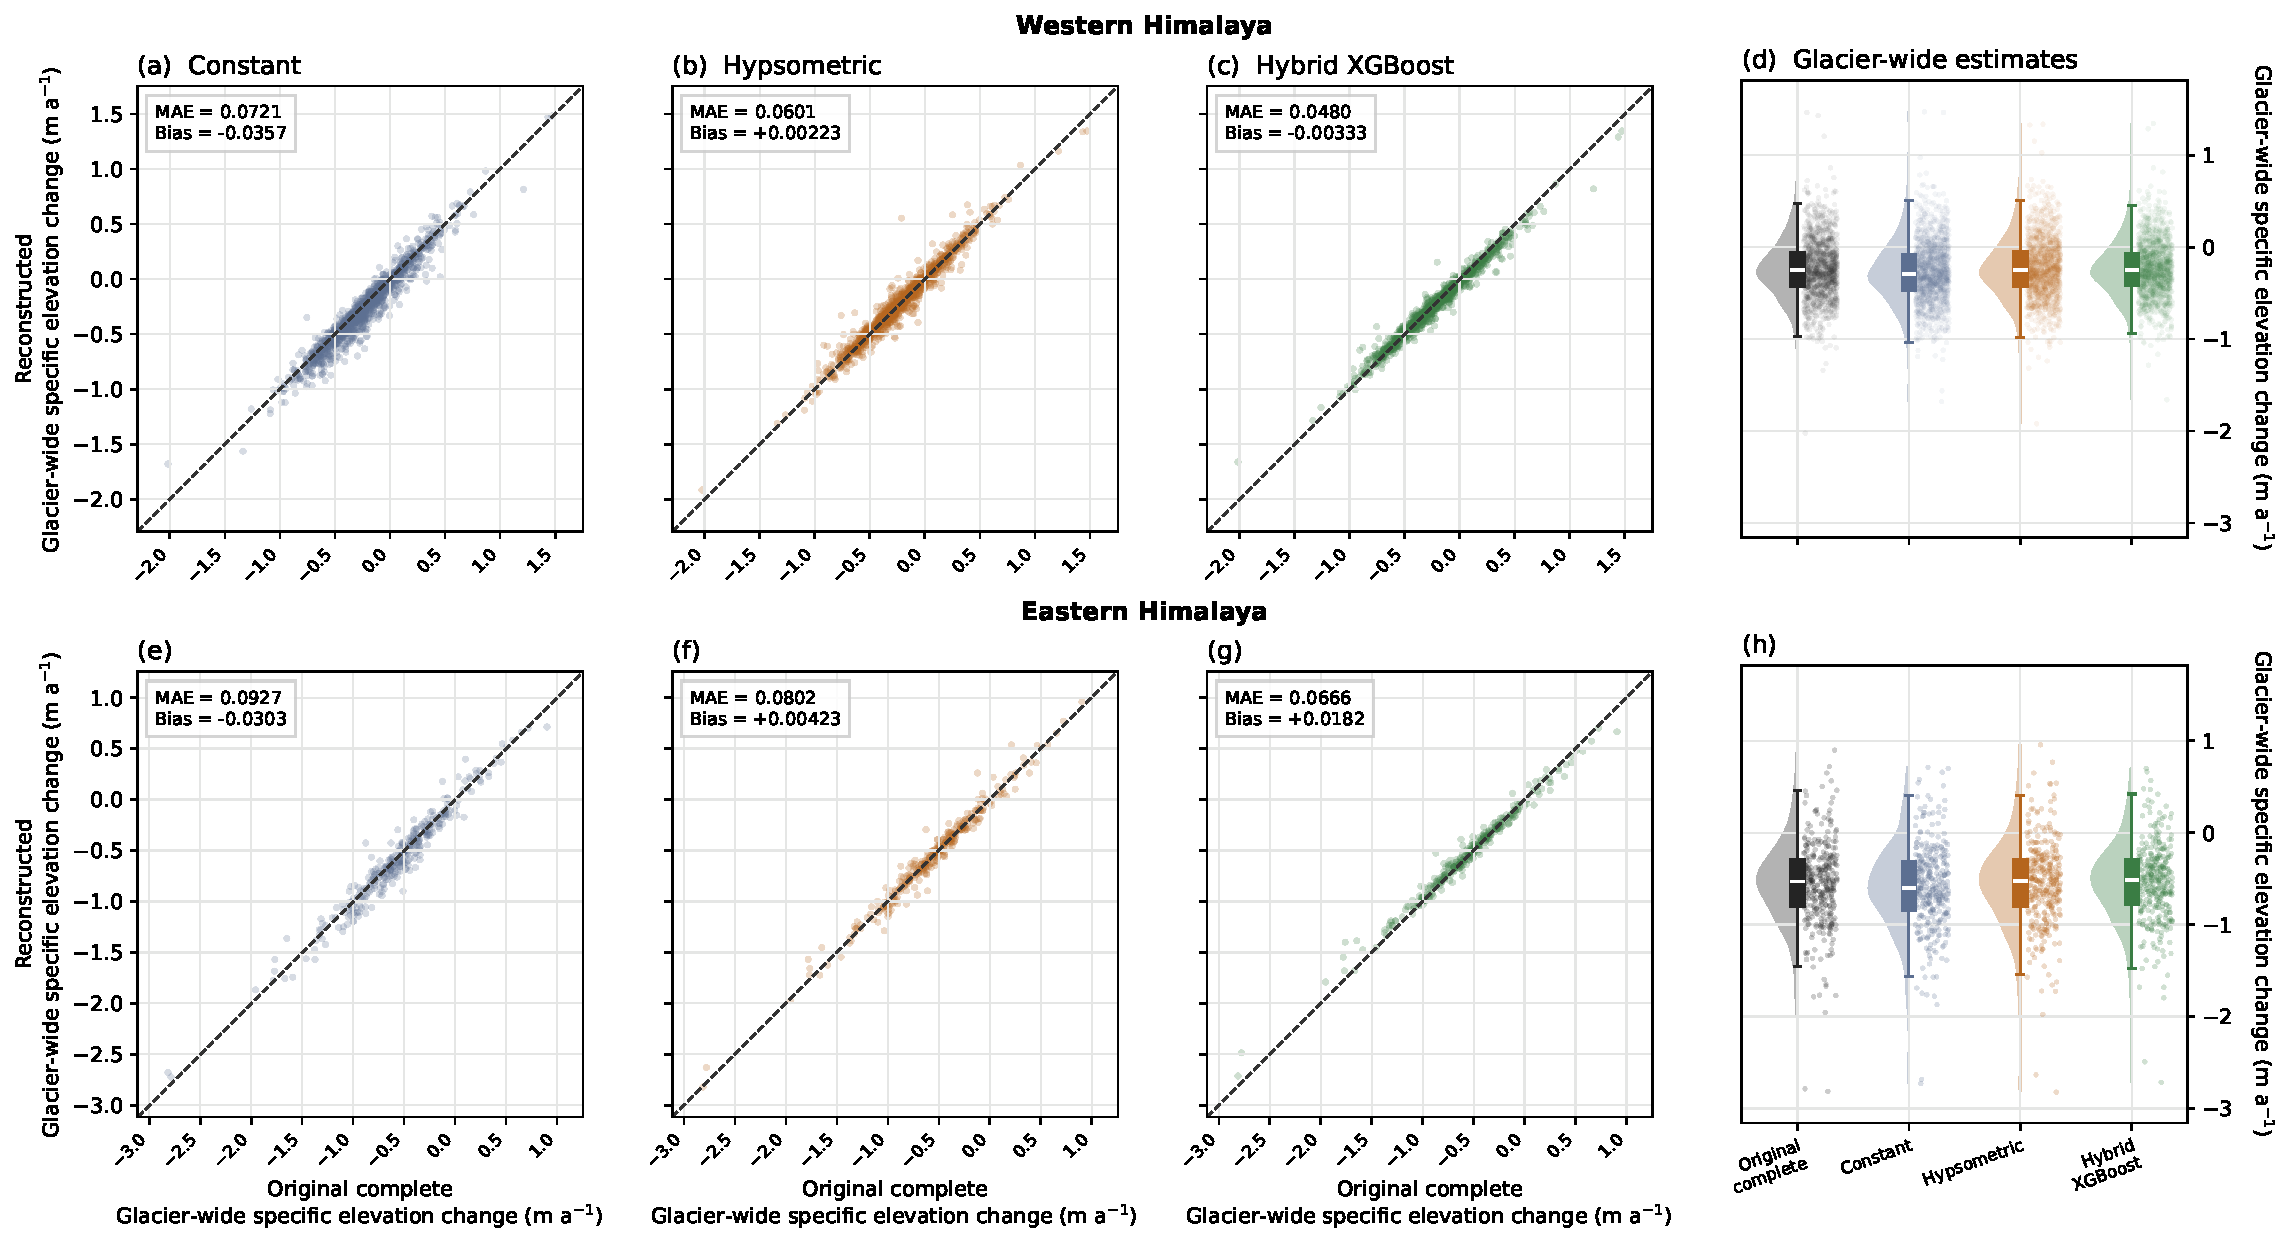
\includegraphics[width=\textwidth,height=.62\textheight,keepaspectratio]{fig05_glacier_wide.pdf}\caption{Reconstructed versus reference glacier-wide specific elevation-change rates for constant, hypsometric, and hybrid filling in the Western (a–c) and Eastern (e–g) Himalaya. Each point represents one of the 1,754 evaluated test glaciers, with reconstructed rates averaged over its five realizations. Dashed diagonals indicate equality. Panels (d,h) combine smoothed distributions, individual glacier points, and boxes showing medians and interquartile ranges. Whiskers extend to the most extreme values within 1.5 interquartile ranges of each box. Observed non-void values are retained in each reconstruction. “Original complete” denotes the available reference-data area before artificial void generation.}\label{fig:glacier}\end{figure}
